\documentclass[a4paper,english]{article}
\usepackage{graphicx}
\usepackage{listings}
\usepackage{amsmath}
\usepackage{multirow}

%% Use utf-8 encoding for foreign characters
%%\usepackage[T1]{fontenc}
%%\usepackage[utf8]{inputenc}
%%\usepackage{babel}
%%
%%%% Vector based fonts instead of bitmaps
%%\usepackage{lmodern}
%%
%%%% Useful
%%%\usepackage{fullpage} % Smaller margins
%%\usepackage{enumerate}
%%
%%%% Theorem
%%\usepackage{amsthm}
%%
%%%% More math
%%\usepackage{amsmath}
%%\usepackage{amssymb}
\lstset{
  breaklines=true,
  postbreak=\mbox{{$\hookrightarrow$}\space},
  numbers=left,
}

%% Document Header
\title{Section3}
\author{Elliott Ashby}
\date{\today}

\begin{document}
    \maketitle
    \section{q1}
    \lstinputlisting[language=Python, firstline=6, lastline=15]{3_1.py}
    The above code first defines the integrad, $f(x)$, and then the function trap0, which takes the integrand, and upper and lower bound and the number of strips to use.
    \section{q2}
    Calling the functions in the following way can calculate the value of the integral.
    \lstinputlisting[language=Python, firstline=67, lastline=78]{3_1.py}
    Running this will give an output for the value of:
    \begin{center}
        $\int_0^1{\frac{x^4(1-x)^4}{1+x^2}dx} = 0.0012649570769764054$
    \end{center}
    \section{q3}
    Which was achieved using 7 strips.
    \section{q4}
    \lstinputlisting[language=Python, firstline=40, lastline=41]{3_1.py}
    \lstinputlisting[language=Python, firstline=80, lastline=80]{3_1.py}
    Which uses the the new traps1 function to calculate the integral. \\
    Continuing to increase this to get precision at 13 sig fig at an integral range of -10 to 10 will calculate:
    \begin{center}
            $\int_{-a}^a{e^{-x^2}dx} = 1.7724538509055157$
    \end{center}
    Where a increases by one every iteration. \\
    Simply running 1 to 10, hence increasing the range of the integral by 2 every time, reveals that results are precise to 12 sig fig at only a range of -5 to 5.
    This produces an output of:
    \begin{lstlisting}
         1.4931691935764426, 1.7639724905315541, 1.7723984788565614, 1.7724537930187396, 1.7724538509008183, 1.7724538509055159, 1.772453850905516, 1.772453850905516, 1.7724538509056167, 1.7724538509055157
    \end{lstlisting}
    \section{q5}
    The integrand of:
    \begin{center}
        $T = T_0\frac{\sqrt{2}}{\pi}\int_0^\alpha\frac{d\theta}{(cos\theta-cos\alpha)^{1/2}}$
    \end{center}
    is:
    \begin{center}
        $\frac{1}{(cos\theta-cos\alpha)^{1/2}}$
    \end{center}
    \lstinputlisting[language=Python, firstline=44, lastline=45]{3_1.py}
    \lstinputlisting[language=Python, firstline=53, lastline=58]{3_1.py}
    \begin{center}
        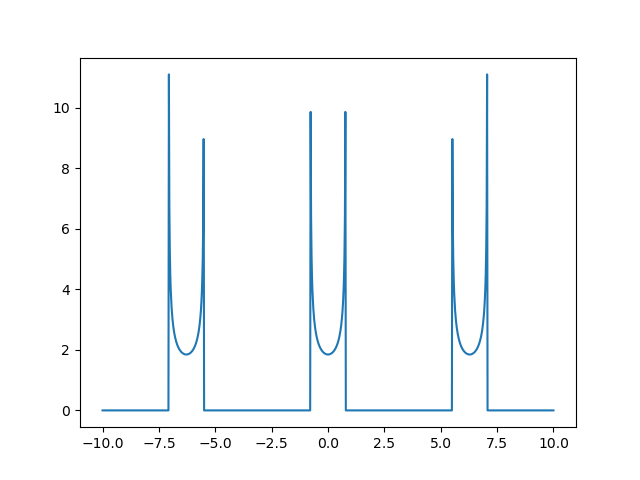
\includegraphics[scale=0.8]{./3_5.png}
        Plot of the output of the integrand against $\alpha$
    \end{center}
    Here, we can see spikes to infinity at values where $\alpha = \theta$. The inconsistent height
    of the asymptotes are because only 1000 discrete value were calculated to graph, meaning that
    these asymptotes are only at $\alpha \approx \theta$.

    We can rewrite the integral as:
    \begin{center}
        $\frac{1}{(1-sin^2(\alpha/2) + sin^2\phi)^{1/2}}$
    \end{center}
    \lstinputlisting[language=Python, firstline=48, lastline=49]{3_1.py}
    \lstinputlisting[language=Python, firstline=60, lastline=63]{3_1.py}
    \begin{center}
        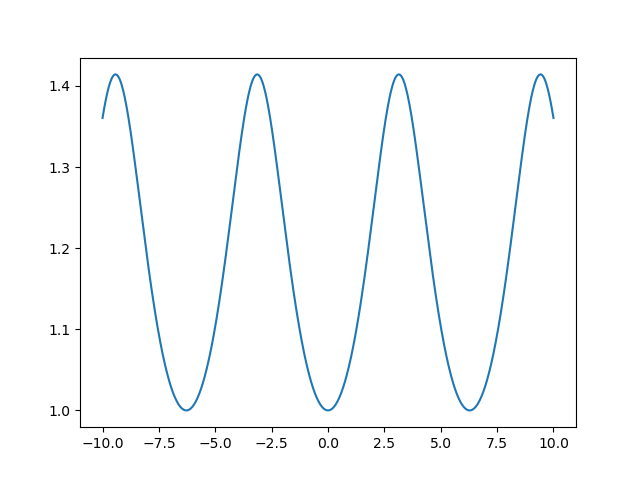
\includegraphics[scale=0.8]{./3_5_2.png}
        Plot of the output of the integrand against $\alpha$
    \end{center}
    \section{q6}
    \lstinputlisting[language=Python, firstline=84, lastline=108]{3_1.py}  
    \begin{center}
        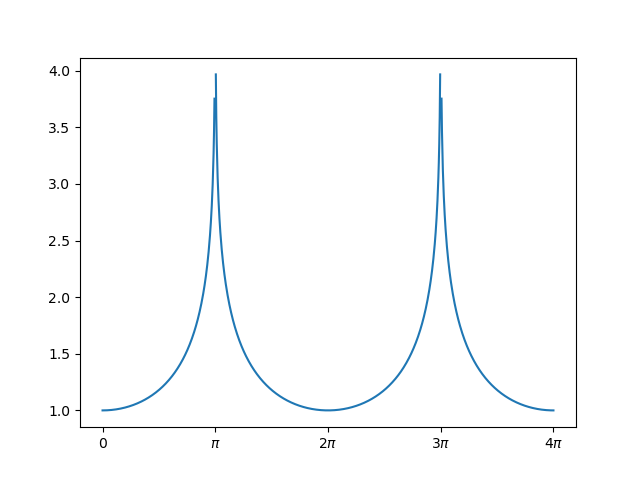
\includegraphics[scale=0.8]{./3_6.png}
        Plot of $T/T_0$ against $\alpha$
    \end{center}
    \section{q7}
    \lstinputlisting[language=Python, firstline=110, lastline=119]{./3_1.py}
        In order to gain a value of $T/T_0$ at $90^\circ$ we simply round both $\pi/2$ and 
        our values of alpha to 2 decimal places, find the index of where $\alpha \approx \pi/2$
        and print the associated ratio.
        \\
        \\
        at $\alpha = 90^\circ$:
    \begin{equation}
        \frac{T}{T_0} = \frac{2}{\pi}\int_0^{\pi/2}\frac{d\phi}{(1-\sin^2(\alpha/2)\sin^2\phi)^{1/2}} 
        = 1.1807649945835401
    \end{equation}
    \section{q8}
    \lstinputlisting[language=Python, firstline=132, lastline=171]{./3_1.py}
    \begin{center}
        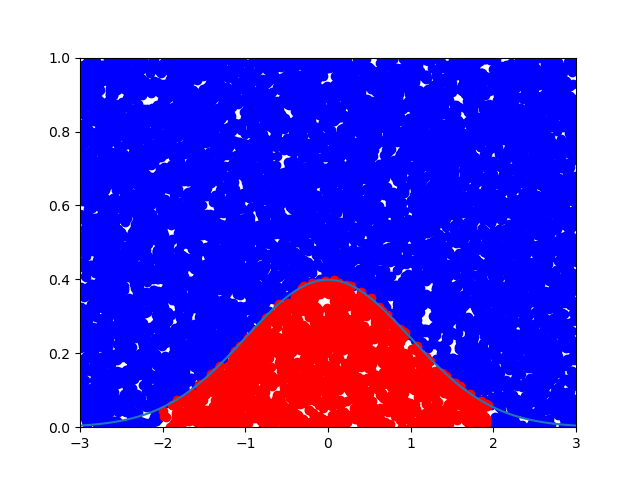
\includegraphics[scale=0.8]{./3_8.png}
        \caption{Random points plotted against a normal distribution, if a points lands within the normal distribution and within $2\sigma$ of the mean it is plotted in red, otherwise blue.}
    \end{center}
    Calculating the number of red points and dividing by the total number of points gives a value of:
    \begin{equation}
        \frac{N_{red}}{N_{total}} = 0.1595
    \end{equation}
    Which, when proportionaly multiplied by the total area of the plot (6), is roughly the same as the area under the normal distribution curve within $2\sigma$ of the mean.
    \begin{equation}
        \frac{N_{red}}{N_{total}} \times 6 = 0.957
    \end{equation}
    Given that the actual value of the area under the normal distribution curve within $2\sigma$ of the mean is 0.9545, this is a very good approximation.
    

\end{document}
